% python classes clides - containers and files
% (c) 2012 Kostiantyn Danylov aka koder 
% koder.mail@gmail.com
% distributed under CC-BY licence
% http://creativecommons.org/licenses/by/3.0/deed.en

\documentclass{article}
% XeLaTeX
\usepackage{xltxtra}
\usepackage{xunicode}
\usepackage{listings}
\usepackage[landscape]{geometry}

% Fonts
\setmainfont{DejaVu Sans} %{Arial}
\newfontfamily\cyrillicfont{Nimbus Roman No9 L} %{Arial}
\setmonofont{Courier New}
%\setmonofont{Ubuntu Mono}

%\setmonofont{DejaVu Sans Mono}

% Lang
\usepackage{polyglossia}
\setmainlanguage{russian}
\setotherlanguage{english}
\usepackage[dvipsnames,table]{xcolor}


\ifx\pdfoutput\undefined
\usepackage{graphicx}
\else
\usepackage[pdftex]{graphicx}
\fi

\lstset{
	language=python,
	keywordstyle=\color{Emerald},%\texttt, 
	commentstyle=\color{OliveGreen},%\texttt,
	stringstyle=\color{Bittersweet},%\texttt,
	tabsize=4,
	numbers=left,
	xleftmargin=10pt,
	morekeywords={with,as},	
	numberstyle=\large,
	%identifierstyle=\texttt,
	%basicstyle=\texttt,
}

\usepackage{hyperref}

\hypersetup{
	colorlinks=true,
	urlcolor=blue
}

\usepackage{float}
%\floatstyle{boxed} 
%\restylefloat{figure}
\usepackage[normalem]{ulem}


\makeatletter
\def\PY@reset{\let\PY@it=\relax \let\PY@bf=\relax%
    \let\PY@ul=\relax \let\PY@tc=\relax%
    \let\PY@bc=\relax \let\PY@ff=\relax}
\def\PY@tok#1{\csname PY@tok@#1\endcsname}
\def\PY@toks#1+{\ifx\relax#1\empty\else%
    \PY@tok{#1}\expandafter\PY@toks\fi}
\def\PY@do#1{\PY@bc{\PY@tc{\PY@ul{%
    \PY@it{\PY@bf{\PY@ff{#1}}}}}}}
\def\PY#1#2{\PY@reset\PY@toks#1+\relax+\PY@do{#2}}

\expandafter\def\csname PY@tok@gd\endcsname{\def\PY@tc##1{\textcolor[rgb]{0.63,0.00,0.00}{##1}}}
\expandafter\def\csname PY@tok@gu\endcsname{\let\PY@bf=\textbf\def\PY@tc##1{\textcolor[rgb]{0.50,0.00,0.50}{##1}}}
\expandafter\def\csname PY@tok@gt\endcsname{\def\PY@tc##1{\textcolor[rgb]{0.00,0.25,0.82}{##1}}}
\expandafter\def\csname PY@tok@gs\endcsname{\let\PY@bf=\textbf}
\expandafter\def\csname PY@tok@gr\endcsname{\def\PY@tc##1{\textcolor[rgb]{1.00,0.00,0.00}{##1}}}
\expandafter\def\csname PY@tok@cm\endcsname{\let\PY@it=\textit\def\PY@tc##1{\textcolor[rgb]{0.25,0.50,0.50}{##1}}}
\expandafter\def\csname PY@tok@vg\endcsname{\def\PY@tc##1{\textcolor[rgb]{0.10,0.09,0.49}{##1}}}
\expandafter\def\csname PY@tok@m\endcsname{\def\PY@tc##1{\textcolor[rgb]{0.40,0.40,0.40}{##1}}}
\expandafter\def\csname PY@tok@mh\endcsname{\def\PY@tc##1{\textcolor[rgb]{0.40,0.40,0.40}{##1}}}
\expandafter\def\csname PY@tok@go\endcsname{\def\PY@tc##1{\textcolor[rgb]{0.50,0.50,0.50}{##1}}}
\expandafter\def\csname PY@tok@ge\endcsname{\let\PY@it=\textit}
\expandafter\def\csname PY@tok@vc\endcsname{\def\PY@tc##1{\textcolor[rgb]{0.10,0.09,0.49}{##1}}}
\expandafter\def\csname PY@tok@il\endcsname{\def\PY@tc##1{\textcolor[rgb]{0.40,0.40,0.40}{##1}}}
\expandafter\def\csname PY@tok@cs\endcsname{\let\PY@it=\textit\def\PY@tc##1{\textcolor[rgb]{0.25,0.50,0.50}{##1}}}
\expandafter\def\csname PY@tok@cp\endcsname{\def\PY@tc##1{\textcolor[rgb]{0.74,0.48,0.00}{##1}}}
\expandafter\def\csname PY@tok@gi\endcsname{\def\PY@tc##1{\textcolor[rgb]{0.00,0.63,0.00}{##1}}}
\expandafter\def\csname PY@tok@gh\endcsname{\let\PY@bf=\textbf\def\PY@tc##1{\textcolor[rgb]{0.00,0.00,0.50}{##1}}}
\expandafter\def\csname PY@tok@ni\endcsname{\let\PY@bf=\textbf\def\PY@tc##1{\textcolor[rgb]{0.60,0.60,0.60}{##1}}}
\expandafter\def\csname PY@tok@nl\endcsname{\def\PY@tc##1{\textcolor[rgb]{0.63,0.63,0.00}{##1}}}
\expandafter\def\csname PY@tok@nn\endcsname{\let\PY@bf=\textbf\def\PY@tc##1{\textcolor[rgb]{0.00,0.00,1.00}{##1}}}
\expandafter\def\csname PY@tok@no\endcsname{\def\PY@tc##1{\textcolor[rgb]{0.53,0.00,0.00}{##1}}}
\expandafter\def\csname PY@tok@na\endcsname{\def\PY@tc##1{\textcolor[rgb]{0.49,0.56,0.16}{##1}}}
\expandafter\def\csname PY@tok@nb\endcsname{\def\PY@tc##1{\textcolor[rgb]{0.00,0.50,0.00}{##1}}}
\expandafter\def\csname PY@tok@nc\endcsname{\let\PY@bf=\textbf\def\PY@tc##1{\textcolor[rgb]{0.00,0.00,1.00}{##1}}}
\expandafter\def\csname PY@tok@nd\endcsname{\def\PY@tc##1{\textcolor[rgb]{0.67,0.13,1.00}{##1}}}
\expandafter\def\csname PY@tok@ne\endcsname{\let\PY@bf=\textbf\def\PY@tc##1{\textcolor[rgb]{0.82,0.25,0.23}{##1}}}
\expandafter\def\csname PY@tok@nf\endcsname{\def\PY@tc##1{\textcolor[rgb]{0.00,0.00,1.00}{##1}}}
\expandafter\def\csname PY@tok@si\endcsname{\let\PY@bf=\textbf\def\PY@tc##1{\textcolor[rgb]{0.73,0.40,0.53}{##1}}}
\expandafter\def\csname PY@tok@s2\endcsname{\def\PY@tc##1{\textcolor[rgb]{0.73,0.13,0.13}{##1}}}
\expandafter\def\csname PY@tok@vi\endcsname{\def\PY@tc##1{\textcolor[rgb]{0.10,0.09,0.49}{##1}}}
\expandafter\def\csname PY@tok@nt\endcsname{\let\PY@bf=\textbf\def\PY@tc##1{\textcolor[rgb]{0.00,0.50,0.00}{##1}}}
\expandafter\def\csname PY@tok@nv\endcsname{\def\PY@tc##1{\textcolor[rgb]{0.10,0.09,0.49}{##1}}}
\expandafter\def\csname PY@tok@s1\endcsname{\def\PY@tc##1{\textcolor[rgb]{0.73,0.13,0.13}{##1}}}
\expandafter\def\csname PY@tok@sh\endcsname{\def\PY@tc##1{\textcolor[rgb]{0.73,0.13,0.13}{##1}}}
\expandafter\def\csname PY@tok@sc\endcsname{\def\PY@tc##1{\textcolor[rgb]{0.73,0.13,0.13}{##1}}}
\expandafter\def\csname PY@tok@sx\endcsname{\def\PY@tc##1{\textcolor[rgb]{0.00,0.50,0.00}{##1}}}
\expandafter\def\csname PY@tok@bp\endcsname{\def\PY@tc##1{\textcolor[rgb]{0.00,0.50,0.00}{##1}}}
\expandafter\def\csname PY@tok@c1\endcsname{\let\PY@it=\textit\def\PY@tc##1{\textcolor[rgb]{0.25,0.50,0.50}{##1}}}
\expandafter\def\csname PY@tok@kc\endcsname{\let\PY@bf=\textbf\def\PY@tc##1{\textcolor[rgb]{0.00,0.50,0.00}{##1}}}
\expandafter\def\csname PY@tok@c\endcsname{\let\PY@it=\textit\def\PY@tc##1{\textcolor[rgb]{0.25,0.50,0.50}{##1}}}
\expandafter\def\csname PY@tok@mf\endcsname{\def\PY@tc##1{\textcolor[rgb]{0.40,0.40,0.40}{##1}}}
\expandafter\def\csname PY@tok@err\endcsname{\def\PY@bc##1{\setlength{\fboxsep}{0pt}\fcolorbox[rgb]{1.00,0.00,0.00}{1,1,1}{\strut ##1}}}
\expandafter\def\csname PY@tok@kd\endcsname{\let\PY@bf=\textbf\def\PY@tc##1{\textcolor[rgb]{0.00,0.50,0.00}{##1}}}
\expandafter\def\csname PY@tok@ss\endcsname{\def\PY@tc##1{\textcolor[rgb]{0.10,0.09,0.49}{##1}}}
\expandafter\def\csname PY@tok@sr\endcsname{\def\PY@tc##1{\textcolor[rgb]{0.73,0.40,0.53}{##1}}}
\expandafter\def\csname PY@tok@mo\endcsname{\def\PY@tc##1{\textcolor[rgb]{0.40,0.40,0.40}{##1}}}
\expandafter\def\csname PY@tok@kn\endcsname{\let\PY@bf=\textbf\def\PY@tc##1{\textcolor[rgb]{0.00,0.50,0.00}{##1}}}
\expandafter\def\csname PY@tok@mi\endcsname{\def\PY@tc##1{\textcolor[rgb]{0.40,0.40,0.40}{##1}}}
\expandafter\def\csname PY@tok@gp\endcsname{\let\PY@bf=\textbf\def\PY@tc##1{\textcolor[rgb]{0.00,0.00,0.50}{##1}}}
\expandafter\def\csname PY@tok@o\endcsname{\def\PY@tc##1{\textcolor[rgb]{0.40,0.40,0.40}{##1}}}
\expandafter\def\csname PY@tok@kr\endcsname{\let\PY@bf=\textbf\def\PY@tc##1{\textcolor[rgb]{0.00,0.50,0.00}{##1}}}
\expandafter\def\csname PY@tok@s\endcsname{\def\PY@tc##1{\textcolor[rgb]{0.73,0.13,0.13}{##1}}}
\expandafter\def\csname PY@tok@kp\endcsname{\def\PY@tc##1{\textcolor[rgb]{0.00,0.50,0.00}{##1}}}
\expandafter\def\csname PY@tok@w\endcsname{\def\PY@tc##1{\textcolor[rgb]{0.73,0.73,0.73}{##1}}}
\expandafter\def\csname PY@tok@kt\endcsname{\def\PY@tc##1{\textcolor[rgb]{0.69,0.00,0.25}{##1}}}
\expandafter\def\csname PY@tok@ow\endcsname{\let\PY@bf=\textbf\def\PY@tc##1{\textcolor[rgb]{0.67,0.13,1.00}{##1}}}
\expandafter\def\csname PY@tok@sb\endcsname{\def\PY@tc##1{\textcolor[rgb]{0.73,0.13,0.13}{##1}}}
\expandafter\def\csname PY@tok@k\endcsname{\let\PY@bf=\textbf\def\PY@tc##1{\textcolor[rgb]{0.00,0.50,0.00}{##1}}}
\expandafter\def\csname PY@tok@se\endcsname{\let\PY@bf=\textbf\def\PY@tc##1{\textcolor[rgb]{0.73,0.40,0.13}{##1}}}
\expandafter\def\csname PY@tok@sd\endcsname{\let\PY@it=\textit\def\PY@tc##1{\textcolor[rgb]{0.73,0.13,0.13}{##1}}}

\def\PYZbs{\char`\\}
\def\PYZus{\char`\_}
\def\PYZob{\char`\{}
\def\PYZcb{\char`\}}
\def\PYZca{\char`\^}
\def\PYZam{\char`\&}
\def\PYZlt{\char`\<}
\def\PYZgt{\char`\>}
\def\PYZsh{\char`\#}
\def\PYZpc{\char`\%}
\def\PYZdl{\char`\$}
\def\PYZti{\char`\~}
% for compatibility with earlier versions
\def\PYZat{@}
\def\PYZlb{[}
\def\PYZrb{]}
\makeatother

\begin{document}
\LARGE

%-------------------------------------------------------------------------------
\center{Контейнеры}
\begin{itemize}
	\item list == [...]
	\item tuple == (...)
	\item dict == \{a:b, ...\}
	\item set == \{a, b, ....\}
\end{itemize}
\newpage

%-------------------------------------------------------------------------------
\center{list – Список (Массив)}
\begin{itemize}
	\item Упорядоченное множество элементов, доступ по номеру
	\item \lstinline!var = [1, 2, 3]!
	\item Индексация \lstinline!arr[x]!
	\item Срезы 
			\lstinline!arr[frm:to:step]! \\
			\lstinline![arr[frm], arr[frm + step], ....., ]!
	\item Отрицательный индекс - отсчет от конца. x[-1]
	\item Отсутвие индекса - frm -> 0, to -> -1, step -> 1
	\item arr[::-1] - инверсия элементов
	\item arr[:] - копия
\end{itemize}
\newpage

%-------------------------------------------------------------------------------
\center{list – Список (Массив)}
{
\Huge
\begin{flushleft}
$x = [0_{-6}^{0}, 1_{-5}^{1}, 2_{-4}^{2}, 3_{-3}^{3}, 4_{-2}^{4}, 5_{-1}^{5}]$ \\
\vspace{0.5cm}
x[2] == 2 \hspace{2cm}[\textcolor{red}{0, 1,} 2, \textcolor{red}{3, 4, 5}] \\
\vspace{0.5cm}
x[-2] == 4 \hspace{2cm}[\textcolor{red}{0, 1, 2, 3,} 4, \textcolor{red}{5}] \\
\vspace{0.5cm}
x[2:] == [2, 3, 4, 5] \hspace{2cm}[\textcolor{red}{0, 1, }2, 3, 4, 5] \\
\vspace{0.5cm}
x[-2:] == [4, 5] \hspace{2cm}[\textcolor{red}{0, 1, 2, 3,} 4, 5] \\
\vspace{0.5cm}
x[1:-1] == [1, 2, 3, 4] \hspace{2cm}[\textcolor{red}{0,} 1, 2, 3, 4, \textcolor{red}{5}] \\
\vspace{0.5cm}
x[1:-1:2] == [1, 3] \hspace{2cm}[\textcolor{red}{0,} 1, \textcolor{orange}{2,} 3, \textcolor{orange}{4,} \textcolor{red}{5}] \\
\vspace{0.5cm}
x[::-1] == [5, 4, 3, 2, 1, 0] \\
\end{flushleft}
}
\newpage

%-------------------------------------------------------------------------------
\center{list – Операции нам элементам и срезам}
\vspace{15pt}
\begin{lstlisting}
	x = [3, 4, 5, 6]
	x[::2] = [2, 2]  # x == [2, 4, 2, 6]
	x[::2] = 2 # error
	del x[1] # x == [3, 5, 6]
	x = [1, None, True, ["123", 2.4]]
	[1, 2, 3] + ["a", "b"] # [1, 2, 3, "a", "b"]
\end{lstlisting}
\newpage

%-------------------------------------------------------------------------------
\center{Методы списка}
\Large{
\vspace{15pt}
\begin{lstlisting}
	# arr.append(val)
	[1, 2].append(3) == [1, 2, 3]

	# arr.extend(arr2)
	[1, 2].extend([2, 3]) == [1, 2, 2, 3]

	# arr.pop()
	x = [1, 2]
	x.pop() == 2
	print x # [1]

	# arr.insert(pos, val)
	[1, 2].insert(0, "abc") == ["abc", 1, 2]

	[1, 2].index(2) == 1
	[1, 2].reverse() == [2, 1]
	[1, 2, 4, 1, 2, 4, 1, 1].count(1) == 4
	x = [1, 3, 2]
	x.remove(1) # x == [3, 2]
	x.sort() # x == [2, 3]
\end{lstlisting}
}
\newpage

%-------------------------------------------------------------------------------
\center{Изменяемые типы (ссылочные)}
\vspace{15pt}
\begin{lstlisting}
	x = [1, 2, 3]
	y = x
	y.append(1)
	print x => [1, 2, 3, 1]
\end{lstlisting}
\newpage

%-------------------------------------------------------------------------------
\center{Изменяемые типы (ссылочные)}
\vspace{15pt}
\begin{lstlisting}
	x = [["1"], "2"]
	y = x
\end{lstlisting}
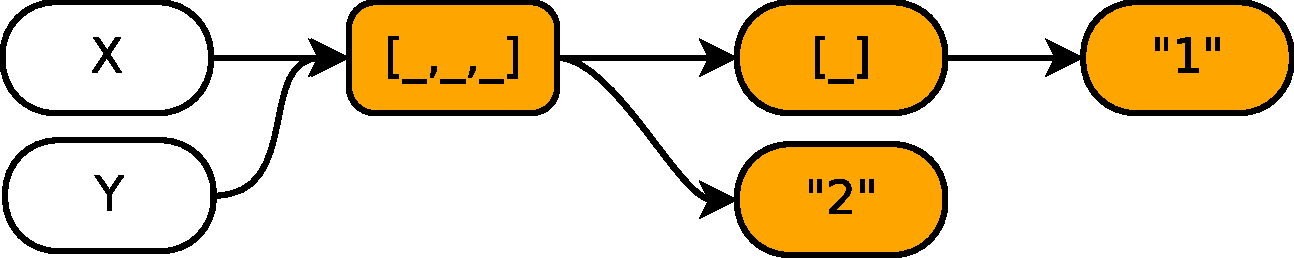
\includegraphics[scale=0.6]{images/refs_1.pdf}

\vspace{15pt}
\begin{lstlisting}
	x = [["1"], "2"]
	y = x[:]
\end{lstlisting}
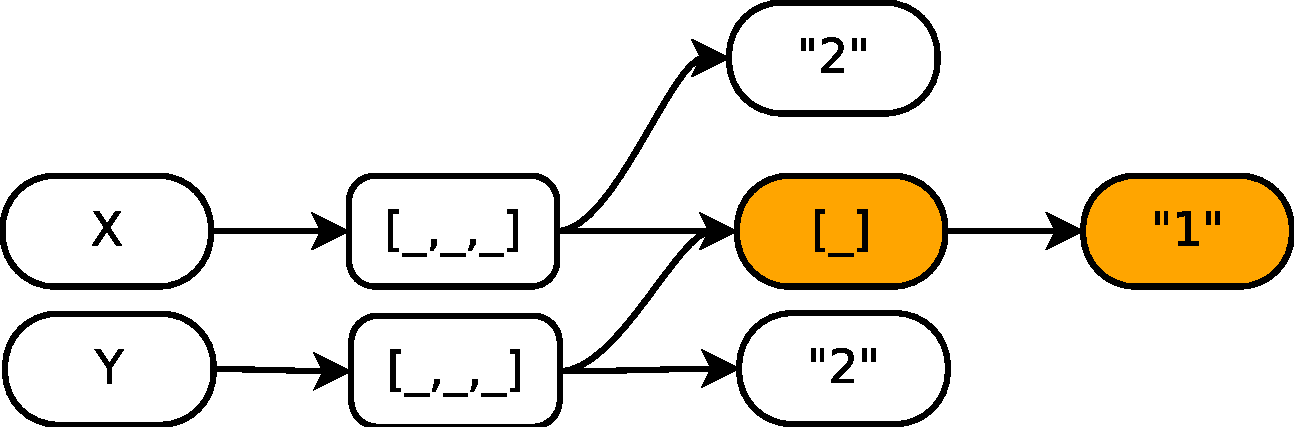
\includegraphics[scale=0.6]{images/refs_2.pdf}

\newpage

\vspace{15pt}
\begin{lstlisting}
	import copy
	x = [["1"], "2"]
	y = copy.deepcopy(x)
\end{lstlisting}
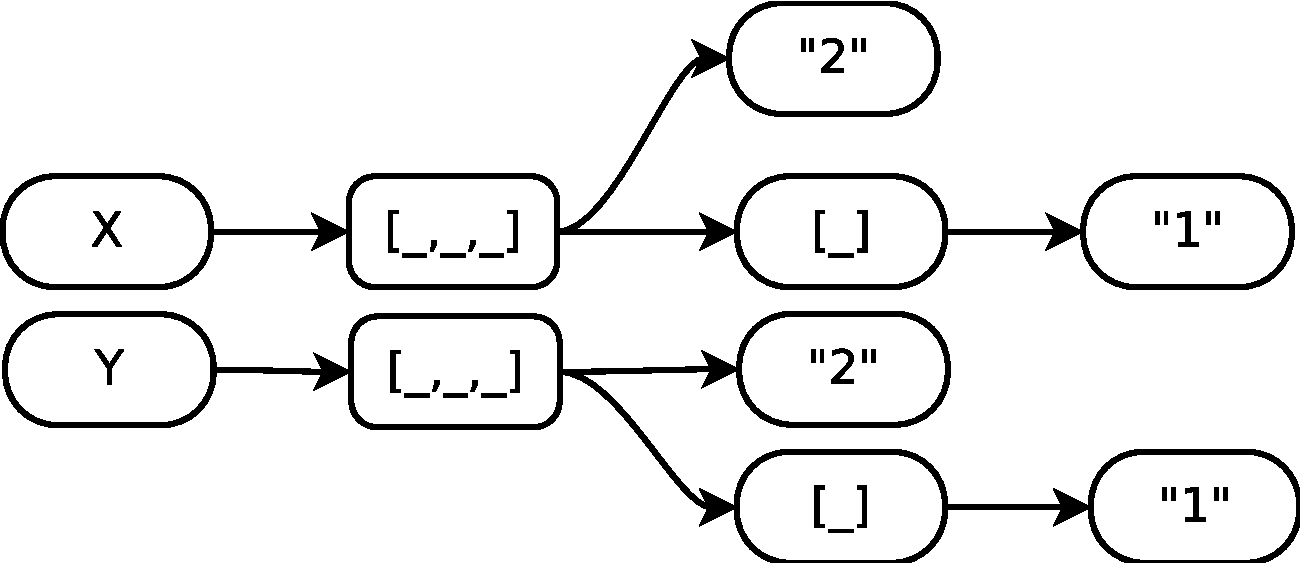
\includegraphics[scale=0.6]{images/refs_3.pdf}

\newpage

%-------------------------------------------------------------------------------
\center{Сортировка}
\begin{itemize}
	\item sort() сортировка на месте, sorted - возвращает копию
	\item sort
	\item Не надо сортировать неоднородные контейнеры типы - результат не определен
		По больше части - получится что-то, но иногда -
		\lstinline!['x', '\xf0', u'x'].sort()! - UnicodeDecodeError
\end{itemize}
\newpage

%-------------------------------------------------------------------------------
\center{tuple – кортеж}
\begin{itemize}
	\item Константный список ( но можно изменять элементы, если они не константные)
\end{itemize}
\vspace{15pt}
\begin{lstlisting}
	tpl = (1, 2)
	tpl = 1,2
	tpl[1] = 3 # error
	tpl = (1, [2, 3, 4])
	tpl[1].append(1) => (1, [2, 3, 4, 1])
	(1) == 1
	(1,) == (1,)
	range(x) == (0, ..., x – 1)
	range(x, y, z) == range(x)[:y:z]
\end{lstlisting}
\newpage

%-------------------------------------------------------------------------------
\center{dict - словарь}
\begin{itemize}
	\item Набор пар (ключ, значение), с быстрым поиском по ключу
	\lstinline$x = {1:2, "3":4}$
	\item Только константные ключи (tuple - ok)
	\item Элементы неупорядоченны
	\item Нет срезов
\end{itemize}
\vspace{15pt}
\begin{lstlisting}
	x[1] == 2
	x[2] #error
	1 in x == True
	x[17] = True
	# x = {1:2, "3":4, 17:True}
\end{lstlisting}
\newpage

%-------------------------------------------------------------------------------
\center{dict – Словарь}
\vspace{15pt}
\begin{lstlisting}
	x = {1:2, "3":"4"}
	dict(a=1, b=2) == {"a":1, "b":2}
	x.items() == [(1, 2), ("3", "4")]
	x.values() == [2, "4"]
	x.keys() == [1, "3"]
	x.copy() == {1:2, "3":"4"}
	x.setdefault(key, val) == val # if key not in x else x[key]
	x.get(5, None) == None # if 5 not in x else x[5]
	x.clear() # {}
	x.update(y)
	dict.fromkeys(keys, val) # {key[0]:val, key[1]:val, ..} default val is None
\end{lstlisting}
\newpage

%-------------------------------------------------------------------------------
\center{set - множество}
\begin{itemize}
	\item Множество элементов с быстрым поиском и операциями
\end{itemize}
\vspace{15pt}
\begin{lstlisting}
	x = {1, 2} 
	y = set([2, "a"]) # y == {2, "a"}
	x & y == x.intersection(y) == {2}
	x – y == x.difference(y) == {1}
	x | y == x.union(y) == {1, 2, "a"}
	x.issubset(y) # ....


	set(1, 2, 3) # error
	set("abcd") == set(["a", "b", "c", "d"])
\end{lstlisting}
\newpage

%-------------------------------------------------------------------------------
%level=3
\center{Особенности поведения set \& dict}
\begin{itemize}
	\item Ключи сравниваются с помощью hash, затем ==
	\item \lstinline!hash(2.0) == 2, hash(2) == 2, 2.0 == 2!
	\item Для пользовательских объектов hash \& == можно перегрузить
\end{itemize}
\begin{lstlisting}
	{2.0: "ccc", 2: "dd"} == {2.0: "ccc"}
	set([2]) | set([2.0]) == set([2])
	set([2.0]) | set([2]) == set([2.0])
	set([2]) == set([2.0])
\end{lstlisting}
\newpage

%-------------------------------------------------------------------------------
\center{Общие операции над контейнерами}
\begin{itemize}
	\item list, tuple, set
	\item len длинна 
	\item str.join \lstinline!", ".join(["1", "2", "3"]) == "1, 2, 3"! 
	\item in проверка включения элемента
	\item dict из [(key1, val1), (key2, val2), …]
\end{itemize}
\newpage

%-------------------------------------------------------------------------------
\center{Циклические контейнеры}
\vspace{15pt}
\begin{lstlisting}
	a = []
	a.append(a)
\end{lstlisting}
\newpage

%-------------------------------------------------------------------------------
\center{Файлы}
\begin{itemize}
	\item Абстракция для источников или приемников данных
	\item Тестовые и бинарные
	\item Можно писать и читать (+os.ioctl)
\end{itemize}
\vspace{15pt}
\begin{lstlisting}
    fd = open(path, mode)
    mode in {"r", "w", "r+", "a", 
             "rb", "wb", "rb+", "ab"}
\end{lstlisting}
\newpage

%-------------------------------------------------------------------------------
\center{Файлы}
\vspace{15pt}
\begin{lstlisting}
	import os
	fd.read(size) # data str
	fd.write("data")
	fd.seek(pos, frm)
	
	# frm in {os.SEEK_SET, os.SEEK_CUR, os.SEEK_END}
	
	fd.read() # till the end
	fd.readline() # untill "\n"
\end{lstlisting}
\newpage
%-------------------------------------------------------------------------------
\end{document}
